\chapter*{Dodatak: Prikaz aktivnosti grupe}
		\addcontentsline{toc}{chapter}{Dodatak: Prikaz aktivnosti grupe}
		
		\section*{Dnevnik sastajanja}
		
		\begin{packed_enum}
			\item  sastanak
			
			\item[] \begin{packed_item}
				\item Datum: 27. listopada 2021.
				\item Prisustvovali: Luka Ivanković, Ante Perković, Lukas Ujčić, Florijan Rusac, Krunoslav Zadrić, Leon Banko
				\item Teme sastanka:
				\begin{packed_item}
					\item  Upoznavanje sa GitLabom
				\end{packed_item}
			\end{packed_item}
			
			\item  sastanak
			\item[] \begin{packed_item}
				\item Datum: 28. listopada 2021.
				\item Prisustvovali: Luka Ivanković, Ante Perković, Lukas Ujčić, Florijan Rusac, Krunoslav Zadrić, Leon Banko, Mario Galić 
				\item Teme sastanka:
				\begin{packed_item}
					\item  Zadavanje zadataka
				\end{packed_item}
			\end{packed_item}

			\item  sastanak
			\item[] \begin{packed_item}
				\item Datum: 31. listopada 2021.
				\item Prisustvovali: Luka Ivanković, Ante Perković, Lukas Ujčić, Florijan Rusac, Krunoslav Zadrić, Leon Banko, Mario Galić 
				\item Teme sastanka:
				\begin{packed_item}
					\item  Provjera napretka i odrađenog
				\end{packed_item}
			\end{packed_item}

			\item  sastanak
			\item[] \begin{packed_item}
				\item Datum: 7. studenoga 2021.
				\item Prisustvovali: Luka Ivanković, Ante Perković, Lukas Ujčić, Florijan Rusac, Krunoslav Zadrić, Leon Banko, Mario Galić 
				\item Teme sastanka:
				\begin{packed_item}
					\item  Provjera napretka i odrađenog
					\item Zadavanje zadataka
				\end{packed_item}
			\end{packed_item}
			
			%
			
		\end{packed_enum}
		
		\eject
		\section*{Tablica aktivnosti}
		

			


			\begin{longtblr}[
					label=none,
				]{
					vlines,hlines,
					width = \textwidth,
					colspec={X[7, l]X[1, c]X[1, c]X[1, c]X[1, c]X[1, c]X[1, c]X[1, c]}, 
					vline{1} = {1}{text=\clap{}},
					hline{1} = {1}{text=\clap{}},
					rowhead = 1,
				} 
				\multicolumn{1}{c|}{} & \multicolumn{1}{c|}{\rotatebox{90}{\textbf{Luka ivanković}}} & \multicolumn{1}{c|}{\rotatebox{90}{\textbf{Lukas Ujčić }}} &	\multicolumn{1}{c|}{\rotatebox{90}{\textbf{Ante Perković }}} & \multicolumn{1}{c|}{\rotatebox{90}{\textbf{Florijan Rusac }}} &	\multicolumn{1}{c|}{\rotatebox{90}{\textbf{Krunoslav Zadrić }}} & \multicolumn{1}{c|}{\rotatebox{90}{\textbf{Mario Galić }}} &	\multicolumn{1}{c|}{\rotatebox{90}{\textbf{Leon Banko }}} \\  
				Upravljanje projektom 		&  &  &  &  &  &  & \\ 
				Opis projektnog zadatka 	&  &  &  &  &  & 2 & \\ 
				
				Funkcionalni zahtjevi       &  &  &  &  &  &  &  \\ 
				Opis pojedinih obrazaca 	&  &  &  & 4 & 4 &  &  \\ 
				Dijagram obrazaca 			&  & 2 &  &  &  &  & 2 \\ 
				Sekvencijski dijagrami 		&  & 3 &  &  &  &  & 4 \\ 
				Opis ostalih zahtjeva 		&  &  &  &  &  & 2 &  \\ 

				Arhitektura i dizajn sustava	 &  &  &  & 1 &  &  &  \\ 
				Baza podataka				&  &  & 5 & 8 & 4 &  &   \\ 
				Dijagram razreda 			&  & 5 &  &  &  &  & 5  \\ 
				Dijagram stanja				&  & 3 &  &  &  &  &  \\ 
				Dijagram aktivnosti 		&  &  &  &  &  &  & 3 \\ 
				Dijagram komponenti			&  &  &  &  &  &  & 1 \\ 
				Korištene tehnologije i alati 		&  &  &  &  &  &  & 1 \\ 
				Ispitivanje programskog rješenja 	&  & 2 & 5 & 3 &  &  & 6 \\ 
				Dijagram razmještaja			&  & 1 &  &  &  &  &   \\ 
				Upute za puštanje u pogon 		&  & 2 &  & 1 &  &  &  \\  
				Dnevnik sastajanja 			&  &  &  &  &  & 0.5 &  \\ 
				Zaključak i budući rad 		&  &  &  &  &  &  &  \\  
				Popis literature 			&  &  &  &  &  &  &  \\  
				&  &  &  &  &  &  &  \\ \hline 
				front end					&  & 4 &  &  &  &  &  \\ 
				Deploy na Heroku 				&  & 11 &  &  &  &  & 5 \\  
				back end 							&  &  & 40 & 25 &  &  & 8 \\  
			\end{longtblr}
					
					
		\eject
		\section*{Dijagrami pregleda promjena}
		\begin{figure}[H]
			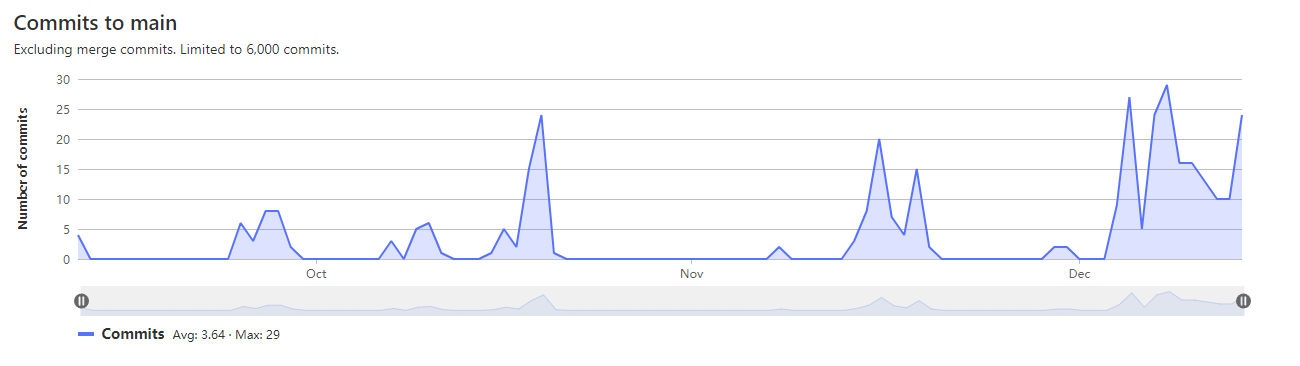
\includegraphics[scale=0.5]{slike/git.png}
			\centering
			\caption{Dijagram pregleda promjena}
			\label{fig:gitlab}
		\end{figure}

		
	
